\newpage
\section{TCP versions}

\subsection{TCP Tahoe}

Characteristics:

\begin{itemize}
  \item Standard TCP functions
  \item ``Slow'' start
  \item Congestion control: AIMD, only timeouts to detect losses (no dupacks)
\end{itemize}

\begin{figure}[H]
  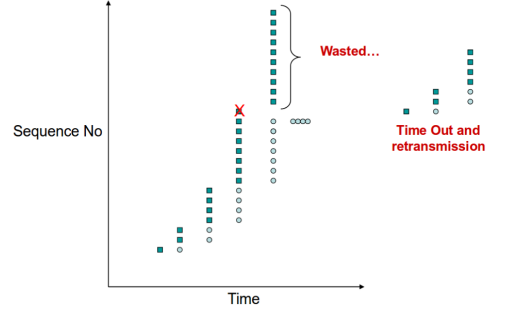
\includegraphics[scale=0.8]{tahoe}
  \caption{TCP Tahoe uses only timeouts to detect losses}
\end{figure}

\subsection{TCP Reno}

Characteristics:

\begin{itemize}
  \item Fast Retransmit/Fast Recovery (3 dupAcks to recover one packet loss)
  \item TCP Reno can recover from one packet loss without having a time out
\end{itemize}

\begin{figure}[H]
  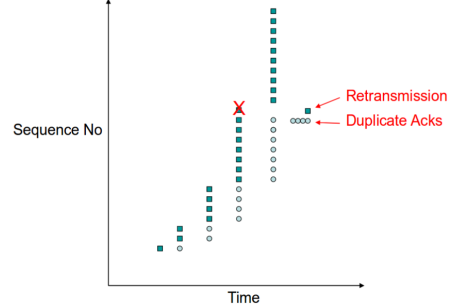
\includegraphics[scale=0.8]{fast_retransmit}
  \caption{TCP Reno - Fast Retransmission}
\end{figure}

\begin{figure}[H]
  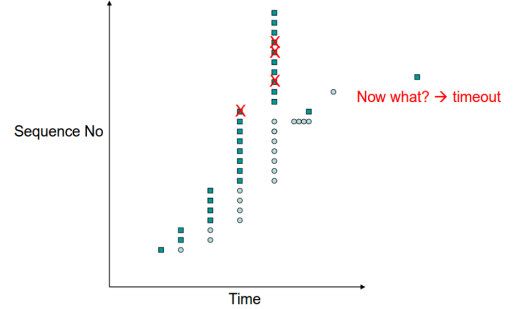
\includegraphics[scale=0.8]{reno}
  \caption{TCP Reno - more than one packet loss}
\end{figure}

\subsubsection{TCP New Reno}

TCP New Reno introduces partial ACKs to recover more packets without the use of
timeouts.

\begin{figure}[H]
  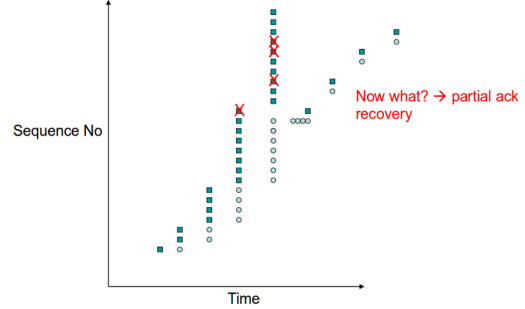
\includegraphics[scale=0.8]{partial_acks}
  \caption{TCP New Reno - partial ACKs}
\end{figure}

\subsection{TCP SACK}

SACK = Selective acknowledgment.

Returning acks declares which packets (even non contiguous) were received.

All non-received packets can be retransmitted and so it recovers from multiple
losses in just one RTT.

\begin{figure}[H]
  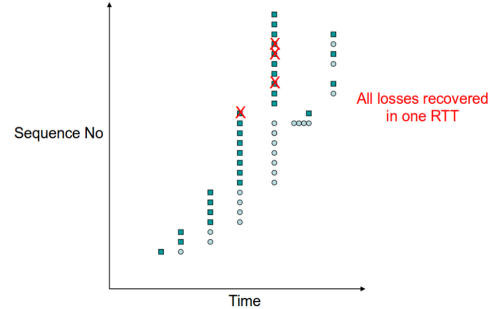
\includegraphics[scale=0.8]{sack}
  \caption{TCP SACK - Recovery from multiple losses in just one RTT}
\end{figure}

\subsection{Congestion control functionality}

$\diamond$ \textbf{Until $cwnd \leq SS\_threshold \rightarrow$} \textbf{SS phase}
(exponential growth)

For each returning ACK, a new packet is transmitted ($cwnd \rightarrow
cwnd + 1$).

For every RTT ($cwnd \rightarrow 2 * cwnd$) \\

$\diamond$ \textbf{When $cwnd > slow\_start\_threshold \rightarrow$}
\textbf{Congestion avoidance phase} (linear growth)

For each returning ACK, a new packet is transmitted ($cwnd \rightarrow
cwnd + (\frac{1}{cwnd})$).

For every RTT ($cwnd \rightarrow cwnd + 1$) \\

\subsection{Loss recovery}

There are two ways to detect losses: time outs and three dupacks.

With timeout expiration:

\begin{itemize}
  \item $ssthresh = \frac{cwnd}{2}$
  \item cwnd = 1 (so, restart in SS phase)
\end{itemize}

With three dupacks:

\begin{itemize}
  \item $ssthresh = \frac{cwnd}{2}$
  \item cwnd = cwnd / 2 (so, restart in cong. avoidance phase)
\end{itemize}

\subsection{TCP Summary}

\begin{figure}[H]
  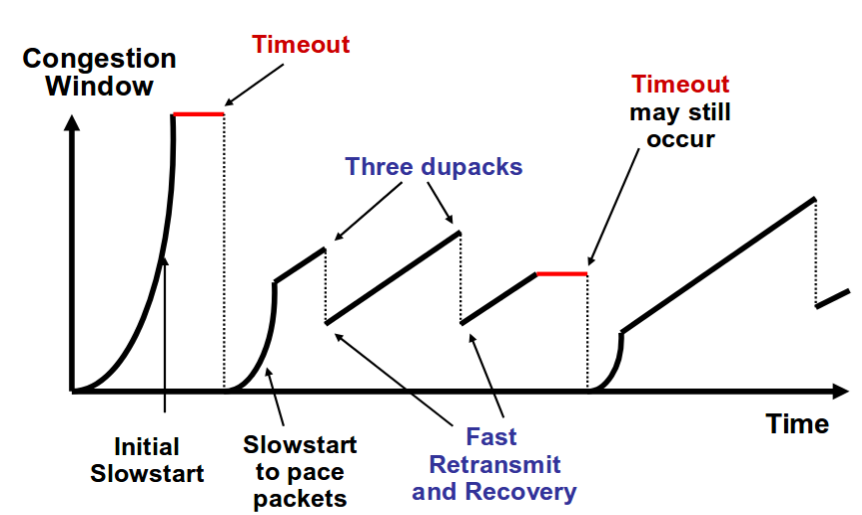
\includegraphics[scale=0.35]{sawTooth}
  \caption{TCP Saw Tooth shape}
  \label{img:sawTooth}
\end{figure}

In figure \ref{img:sawTooth} it's possible to notice the cwnd behaviour with
timeouts, three dupAcks and the changes between SS phase and CA phase.
